In this chapter, we look at how the XYZ technique formulated in Chapter~\ref{cha:main_chapter} can be applied to different scenarios involving ABC. Through a series of examples, we will see the versatility of the MNP technique and how it can be used to ABC. \newline

In this chapter, we automate the given examples using the XYZ tool. For more information regarding the use of the XYZ tool, refer to Appendix~\ref{app:relview}.


\section{Application One}
\label{sec:app_one}
% Begin Section

We continue with the illustrative example introduced in Section~\ref{sec:the_proposed_technique}. Lorem ipsum dolor sit amet, consectetur adipiscing elit. Cras et nibh vel mauris pharetra viverra. Integer nisl nibh, ullamcorper eget imperdiet sed, accumsan ultrices purus. Quisque malesuada vel elit in cursus. Vestibulum rutrum turpis sed lectus vehicula, et venenatis ligula varius. Vivamus auctor fermentum libero, in ullamcorper diam pulvinar non. Donec condimentum cursus iaculis. Nulla odio dolor, faucibus eget mauris a, eleifend congue erat. Interdum et malesuada fames ac ante ipsum primis in faucibus. Nullam aliquet finibus ligula eu feugiat. Aenean feugiat nunc et arcu elementum vestibulum. \newline  

Through Example~\ref{ex:single_channel} we will show that nulla vulputate ultricies felis, ut feugiat nisl auctor a. Lorem ipsum dolor sit amet, consectetur adipiscing elit. \newline

\begin{example}~
\label{ex:single_channel}
	Consider a case where the set of confidential information is represented as $P = \set{(1,3),(2,1),(3,4),(4,1),(5,5),(6,9)}$. Suppose that \AgentOne sends this information encrypted over a single communication channel as $Q = \set{(1,12),(2,1),\\(3,16),(4,1),(5,17),(6,18)}$. \newline 
	
	We define the relations $P$ and $Q$ in \relview\ as follows: \newline
	
	\begin{figure}[ht]
		\centering
		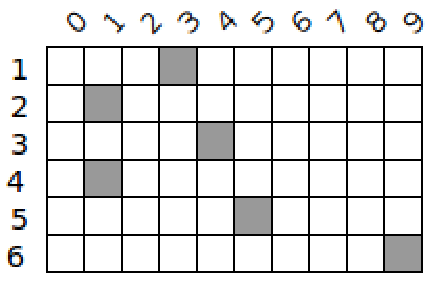
\includegraphics[scale=0.65]{Figures/PDF/Relview/P.pdf}
		\caption{Relation $P$ for Example~\ref{ex:single_channel}.}
		\label{fig:single_channel_p}
	\end{figure}
	
	\begin{figure}[ht]
		\centering
		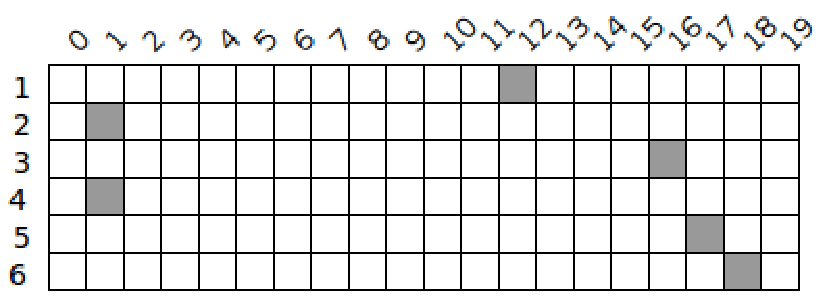
\includegraphics[scale=0.65]{Figures/PDF/Relview/Q.pdf}
		\caption{Relation $Q$ for Example~\ref{ex:single_channel}.}
		\label{fig:single_channel_q}
	\end{figure}	
	
	We verify the existence of an abstraction relation by applying Corollary~\ref{cor:test} using \relview. By executing Program~\ref{prog:test} ($Result = Test(P,Q)$), we obtain the following result: \newline
	
	\begin{figure}[ht]
		\centering
		
\includegraphics[scale=0.65]{Figures/PDF/Relview/True.pdf}
		\caption{Relation $Result$ for Example~\ref{ex:single_channel}.}
		\label{fig:single_channel_result}
	\end{figure}

	Therefore, the test has passed meaning that there exists an abstraction relation relating the confidential information to the information observed to be sent on the communication channel. This means that we can apply Corollary~\ref{cor:compute} by executing Program~\ref{prog:compute} ($X = Compute(P,Q,\RAtop)$) to obtain the abstraction relation, $X$. \newline

	\begin{figure}[ht]
		\centering
		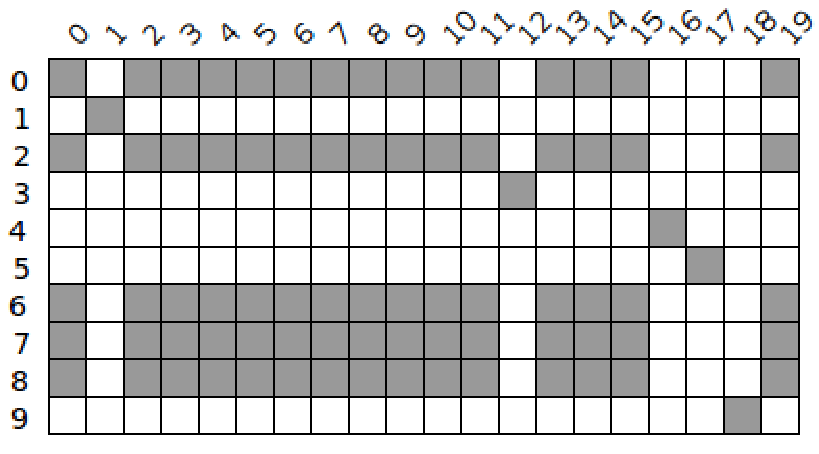
\includegraphics[scale=0.65]{Figures/PDF/Relview/X.pdf}
		\caption{Abstraction relation $X$ for Example~\ref{ex:single_channel}.}
		\label{fig:single_channel_x}
	\end{figure}

	From this result, we can see that there are some digits which are related to information which we do not necessarily have an interest in, \ie we are only concerned with the confidential information which consists of the digits $1,3,4,5, \text{ and } 9$. Therefore we can design a filter $R$ which can be used to refine the abstraction relation $X$. We define $R$ in \relview\ as follows: \newline
	
	\begin{figure}[ht]
		\centering
		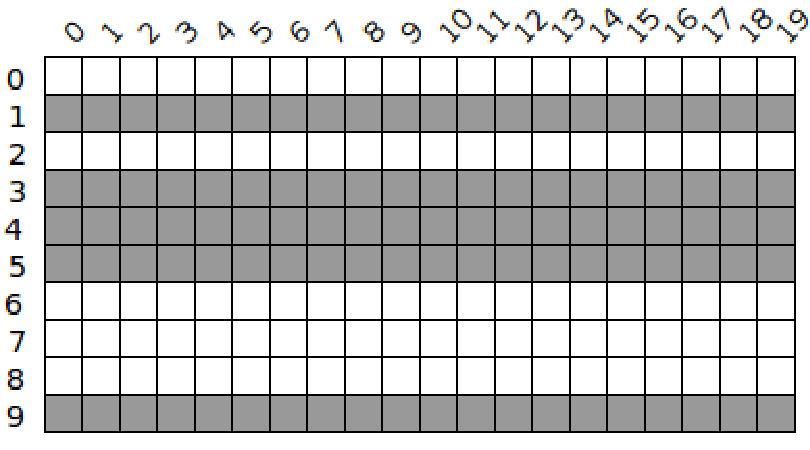
\includegraphics[scale=0.65]{Figures/PDF/Relview/R.pdf}
		\caption{Filtering relation $R$ for Example~\ref{ex:single_channel}.}
		\label{fig:single_channel_r}
	\end{figure}
	
	By executing Program~\ref{prog:compute} with the filter $R$, ($X_{filtered} = Compute(P,Q,R)$), we obtain the abstraction relation, $X_{filtered}$ \newline
	\vspace{-0.25in}
	\begin{figure}[ht]
		\centering
		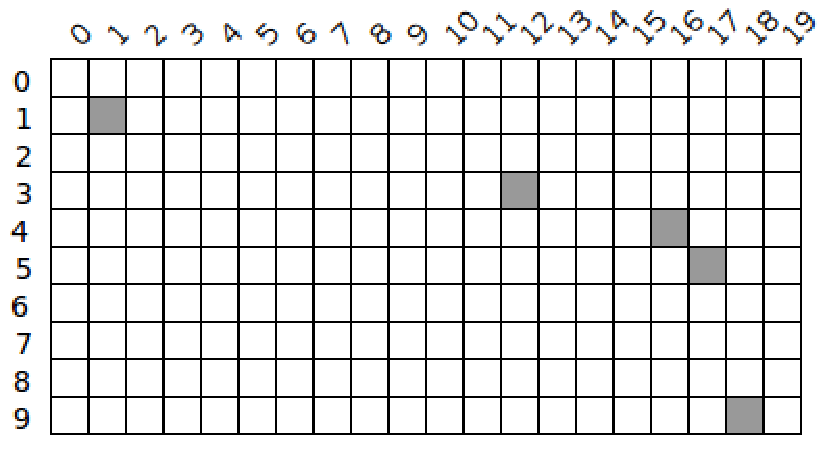
\includegraphics[scale=0.65]{Figures/PDF/Relview/XR.pdf}
		\caption{Abstraction relation $X_{filtered}$ for Example~\ref{ex:single_channel}.}
		\label{fig:single_channel_xr}
	\end{figure}
	 
\end{example}

% End Section

\section{App Two}
\label{sec:app_two}
% Begin Section

Pellentesque vitae imperdiet mi, vel semper arcu. Sed venenatis molestie elit, at malesuada sem suscipit non. In et tristique elit, sit amet aliquet arcu. Maecenas enim ex, aliquam nec diam vel, gravida tristique risus. Integer massa augue, porta sed dui quis, efficitur venenatis arcu. Sed massa dolor, auctor vitae felis eu, mollis mollis neque. Nunc luctus, sapien et auctor faucibus, justo metus ultricies nulla, nec consequat augue magna quis quam. Curabitur tristique bibendum vehicula. Sed quis dictum odio. Donec eget vestibulum sem. Nullam facilisis libero vel justo mattis luctus. Suspendisse auctor fringilla mi non varius. Proin vitae quam massa. Nam sit amet tristique urna, quis pharetra diam. Cras efficitur enim sed accumsan imperdiet. Vivamus euismod non odio nec semper. \newline

Sed quis tellus maximus, condimentum mauris at, dictum diam. Curabitur faucibus, velit id vulputate facilisis, turpis quam molestie mi, ac imperdiet diam nisi ut tellus. Etiam ultrices orci at ante convallis, in rhoncus lacus posuere. Nam vel ullamcorper leo, eu aliquet ante. Cras venenatis sagittis mauris efficitur fringilla. Maecenas at pretium arcu. Duis rhoncus lorem metus, quis laoreet eros porttitor vitae. \newline

This idea is best illustrated through Example~\ref{ex:single_modulated}. \newline

\begin{example}~
\label{ex:single_modulated}
	Assume the set of confidential information is given as $P = \set{(1,3),(2,1),(3,4),(4,1),(5,5),(6,9)}$. In order to obscure the transmission of the information, \AgentOne modulates the confidential information by a relation represented by $M = \set{(0,9),(1,0),(2,1),(3,2),(4,3),(5,4),(6,5),(7,6),(8,7),(9,8)}$ prior to its encryption. Then, the new relation representing the confidential information is given by $(\RAcompose{P}{M}) = \set{(1,2),(2,0),(3,3),(4,0),(5,4),(6,8)}$. This information is encrypted and sent on a single communication channel as $Q = \set{(1,11),(2,0),(3,12),(4,0),(5,16),\\(6,8)}$.  \newline 

	We define the relations $P$, $M$ and $Q$ in \relview\ as follows: \newline

	\begin{figure}[ht]
		\centering
		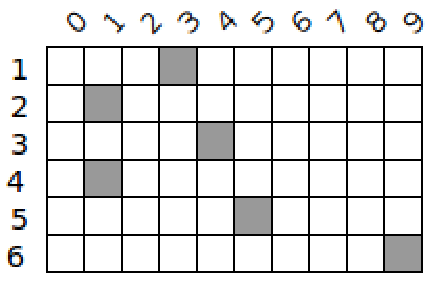
\includegraphics[scale=0.65]{Figures/PDF/Relview/P.pdf}
		\caption{Relation $P$ for Example~\ref{ex:single_modulated}.}
		\label{fig:single_modulated_p}
	\end{figure}
	
	\begin{figure}[ht]
		\centering
		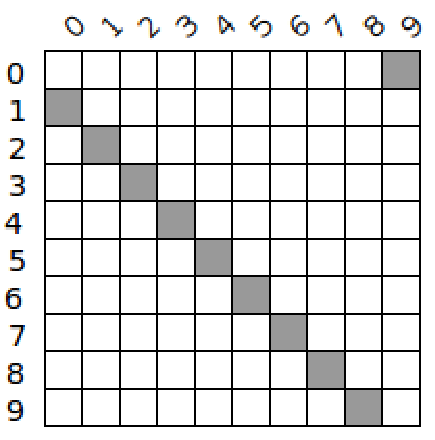
\includegraphics[scale=0.65]{Figures/PDF/Relview/NoiseP.pdf}
		\caption{Modulation relation $M$ for Example~\ref{ex:single_modulated}.}
		\label{fig:single_modulated_s}
	\end{figure}
	
	\begin{figure}[ht]
		\centering
		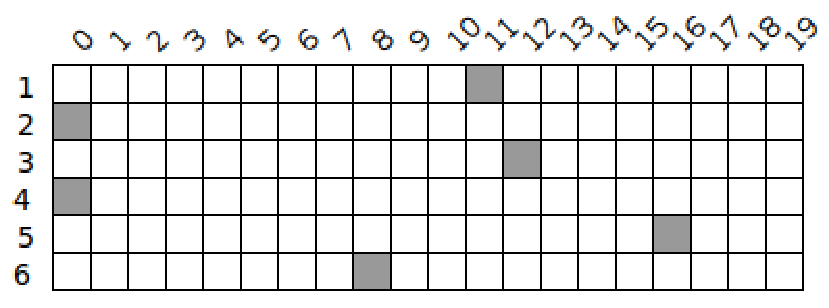
\includegraphics[scale=0.65]{Figures/PDF/Relview/Qmod.pdf}
		\caption{Relation $Q$ for Example~\ref{ex:single_modulated}.}
		\label{fig:single_modulated_q}
	\end{figure}
	\newpage

	The modulated confidential information is represented in \relview\ as follows: \newline
	
	\begin{figure}[ht]
		\centering
		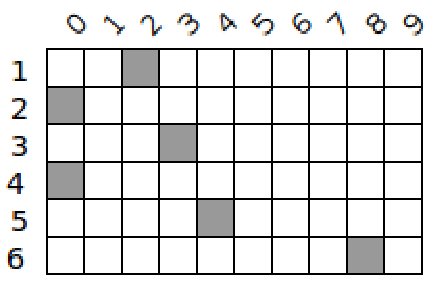
\includegraphics[scale=0.65]{Figures/PDF/Relview/PNoiseP.pdf}
		\caption{Relation $(\RAcompose{P}{M})$ for Example~\ref{ex:single_modulated}.}
		\label{fig:single_modulated_ps}
	\end{figure}
	
	We verify the existence of an abstraction relation by executing Program~\ref{prog:test} ($Result = Test(P, Q)$). In this case we are looking for an abstraction relation relating the confidential information, $P$, and the information sent on the communication channel, $Q$, which corresponds to the encrypted modulated confidential information. \newline

	\begin{figure}[ht]
		\centering
		
\includegraphics[scale=0.65]{Figures/PDF/Relview/True.pdf}
		\caption{Relation $Result$ for Example~\ref{ex:single_modulated}.}
		\label{fig:single_modulated_result}
	\end{figure}

	Therefore, the test has passed so we can compute the abstraction relation by executing Program~\ref{prog:compute} ($X = Compute(P,Q,R)$) where $R$ is the filtering relation. \newline

	\begin{figure}[ht]
		\centering
		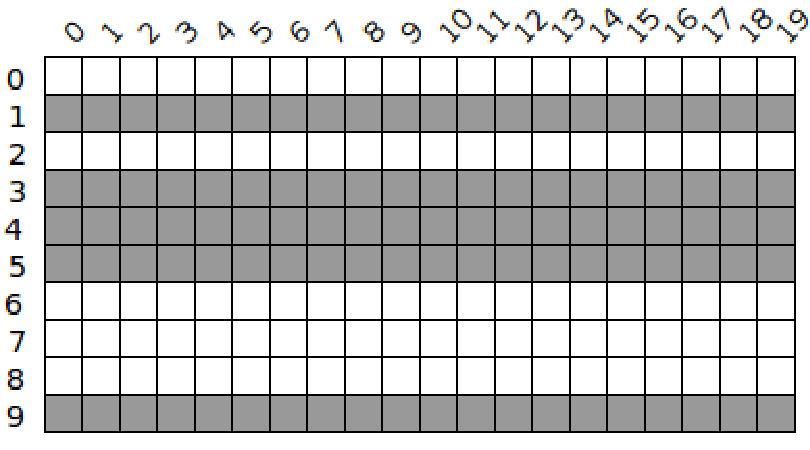
\includegraphics[scale=0.65]{Figures/PDF/Relview/R.pdf}
		\caption{Filtering relation $R$ for Example~\ref{ex:single_modulated}.}
		\label{fig:single_modulated_r}
	\end{figure}
	
	\begin{figure}[ht]
		\centering
		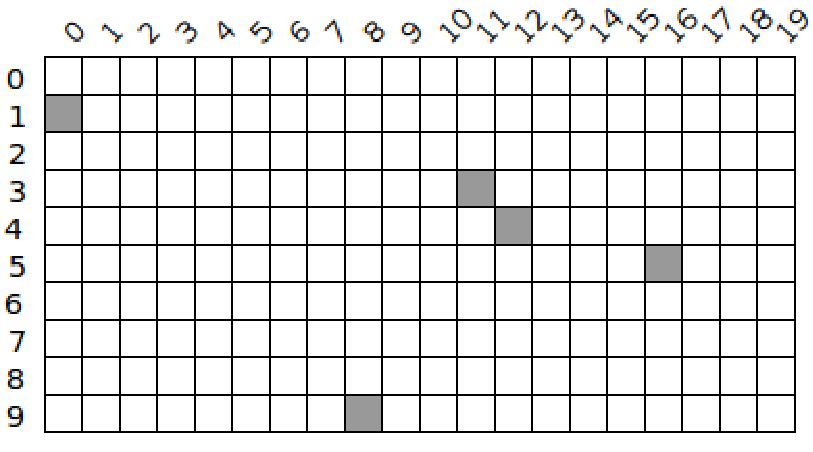
\includegraphics[scale=0.65]{Figures/PDF/Relview/XNP.pdf}
		\caption{Abstraction relation $X$ for Example~\ref{ex:single_modulated}.}
		\label{fig:single_modulated_x}
	\end{figure}
	
	\newpage
\end{example}

% End Section

\section{Conclusion}
\label{sec:application_conclusion}
% Begin Section

In imperdiet purus nec eleifend finibus. Aliquam non tempor massa. Etiam ac felis et ante varius vehicula nec eget tortor. Proin posuere quis felis non rutrum. Aenean quis felis ut ex sagittis pellentesque sit amet tempus nisl. Nam nec tellus ut lorem posuere semper non ac arcu. Nulla faucibus purus libero, in pellentesque sapien commodo tristique. Etiam consectetur lectus elit, id porttitor justo dignissim interdum. Donec ut nisl metus. Nulla sed dui lacus. Donec tristique dignissim massa sed ultricies. Maecenas iaculis arcu diam, ut dictum nisi euismod vitae. Praesent id imperdiet augue.

% End Section